\documentclass[10pt,journal,cspaper,compsoc]{IEEEtran}

\usepackage{graphicx}
\usepackage{amsmath}
\usepackage{url}
\usepackage{mathabx}
\usepackage{tabularx}
\usepackage[numbers]{natbib}
% \usepackage{afterpage}
\newcolumntype{L}[1]{>{\raggedright\arraybackslash}p{#1}}
\newcolumntype{C}[1]{>{\centering\arraybackslash}p{#1}}
\newcolumntype{R}[1]{>{\raggedleft\arraybackslash}p{#1}}


\title{Simulation and Modeling Experiments}
\author{\IEEEauthorblockN{{\bfseries 
  Aayush Lamichhane\IEEEauthorrefmark{1},
  Bishal Katuwal\IEEEauthorrefmark{2},
  Bishant Baniya\IEEEauthorrefmark{3}, and
  Gobind Prasad Sah\IEEEauthorrefmark{4}}}\\
\IEEEauthorblockA{Department of Electronics and Computer Engineering, IOE Pulchowk Campus\\
Patan, Lalitpur\\
Email: \IEEEauthorrefmark{1}075bct005.aayush@pcampus.edu.np,
\IEEEauthorrefmark{2}075bct028.bishal@pcampus.edu.np,
\IEEEauthorrefmark{3}075bct030.bishant@pcampus.edu.np,
\IEEEauthorrefmark{4}075bct038.gobind@pcampus.edu.np,
}}
\date{\today}

\begin{document}
\maketitle

\begin{abstract}
  This report presents the results of five simulation and modeling experiments conducted in both MATLAB and Python. The experiments cover a broad range of topics, including the simulation of a chemical reaction system, an R-C amplifier circuit, the generation of random numbers, the modeling of a mass spring damper system and a national econometric system. The simulations were conducted using mathematical models and software tools, and the results were analyzed and compared with theoritical data, whenever possible. These experiments demonstrate the importance and applications of simulation and modeling in engineering and science, and provide valuable insights into the behavior and performance of complex systems under different scenarios.
\end{abstract}

\section{Introduction}
Simulation and modeling are powerful tools for analyzing and predicting the behavior of complex systems in engineering and science under various scenarios. By creating mathematical models of real-world phenomena, the behaviour of complex systems under different conditions can be simulated. The results provided by simulation can be used to gain insights into the underlying mechanisms of the system. This helps to make predictions about future behavior of the system under consideration.

The remainder of this report is organized as follows. Sections 2 to 6 present the codes, results and discussion regarding the experiments. Section 7 provides a summary of the experiments and their results, and discusses the implications of the findings.

\section{Experiment 1 : Simulation of the chemical reaction}
\subsection{Objectives}
  \begin{itemize}
    \item To develop the mathematical modeling of the continuous system.
    \item To determine the state of the system i.e. the value of reactants and product at different point of
    time.
  \end{itemize}
  \subsection{Methodology}
  Chemical reactions exhibit dynamic equilibrium. At the steady state the rates of the forward and the backward reaction is same.
  in this study, we considered a reaction where two chemicals(C1 and C2) react together to form a third chemical(C3),
  \begin{equation}
    C1 + C2 = C3
  \end{equation} 
  The rate of reaction depends on a large number of factors such as 
  \begin{enumerate}
    \item Amount of C1 and C2 used.
    \item Temperature
    \item Pressure
    \item Humidity
    \item Catalyst
  \end{enumerate}
  For this study, we ignored all other parameters and assume the reaction to only depend on amount of chemicals.
  This allowed the simulation of chemical reaction using ordinary differential equations (ODEs) and/or partial differential equations (PDEs).
  The rate of increase of C1, C2 and C3 at any given instance is given by:
  \begin{equation}
    \frac{dC1}{dt} = K_{2} C3 - K_{1} C1 C2 
  \end{equation}
\begin{equation}
  \frac{dC2}{dt} = K_{2} C3 - K_{1} C1 C2
\end{equation}
\begin{equation}
  \frac{dC3}{dt} = 2 K_{1} C1 C2 - 2 K_{2} C3
\end{equation}
where K1 and K2 are rates of forward and backward reaction respectively.\\
Considering C1(t), C2(t) and C3(t) as the concentration of C1, C2 and C3 at time t, the concentration at time 
\begin{math}
  t + \Delta t
\end{math}
is :
\begin{equation}
  C1(t+\Delta t) = C1(t) + \frac{dC1(t)}{dt} \Delta t
\end{equation} 
\begin{equation}
  C2(t+\Delta t) = C2(t) + \frac{dC2(t)}{dt} \Delta t
\end{equation}
\begin{equation}
  C3(t+\Delta t) = C3(t) + \frac{dC3(t)}{dt} \Delta t
\end{equation}
Using this methodology, the state of the system was simulated.
\cite{lab1}
\pagebreak  
\subsection{Results}
    
    \subsubsection*{Case 1: K1=K2=1, C1[0]=5, C2[0]=2 and C3[0]= 1}
    In this case, forward and backward reaction are equally favoured.
    The simulation shows that since the concentration of reactants is higher than product,
    forward reaction is favoured. Also this continues till the concentration of reactants and products are comparable.
    This is because both forward and backward reaction are equally favoured.
    \begin{figure}[h!]
      \centering
      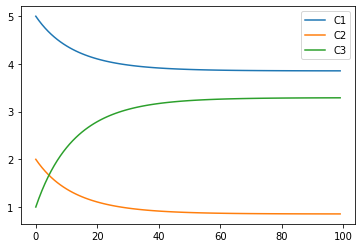
\includegraphics[scale=0.5]{images/Exp1_Example1.png}
      \caption{Kinetics for K1=K2=1, C1[0]=5, C2[0]=2 and C3[0]= 1}
    \end{figure}

    \subsubsection*{Case 2: K1=1, K2=10, C1[0]=5, C2[0]=2 and C3[0]= 10}
    In this case, backward reaction is heavily favoured(K2 = 10) as compared to forward reaction(K1 = 1).
    The simulation shows that since the concentration of product is higher than reactants, backward reaction is favoured. 
    Also this continues even after the concentration of reactants and products are comparable.
    This is because backward reaction is more favoured.
    Since the rate(K2=10) and concentration of product(C3[0]=10) is higher than Case1, the reaction is more rapid.
    \begin{figure}[h!]
      \centering
      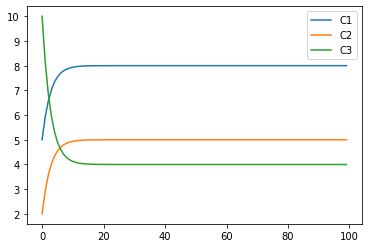
\includegraphics[scale = 0.5]{images/Exp1_Example2.png}
      \caption{Kinetics for K1=1, K2=10, C1[0]=5, C2[0]=2 and C3[0]= 10}
    \end{figure}

    
    \subsubsection*{Case 3: K1=10, K2=1, C1[0]=0, C2[0]=2 and C3[0]= 10}
    In this case, forward reaction is heavily favoured(K1 = 10) as compared to backward reaction(K2 = 1).
    However, the reaction starts with no C1 reactant and high concentration of product(C3[0] = 10). 
    The simulation shows that since the concentration of product is higher than reactants, backward reaction is favoured even though the rate of forward reaction is far greater than backward reaction. 
    This continues only slightly because even though the concentration parity is high, backward reaction isn't favoured and thus the system comes to equilibrium even at that disparity.
    \begin{figure}[h!]
      \centering
      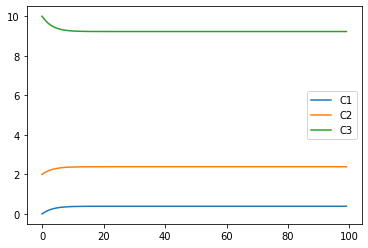
\includegraphics[scale = 0.5]{images/Exp1_Example3.png}
      \caption{Kinetics for K1=10, K2=1, C1[0]=0, C2[0]=2 and C3[0]= 10}
    \end{figure}
    \subsection{Discussion}
    The results of the first experiment showed that the state of the system is highly dependent on the initial concentration of the reactants and the rate of forward and backward reaction.
    In the three cases we studied, forward reaction was preferred when either the concentration of reactant was high or rate of forward reaction was high.
    Similarly, backward reaction was favoured when either the concentration of product was high or the rate of backward reaction was high. 
    Also comparatively, the reaction was faster when the concentration disparity of the chemicals were high.
    Alternatively, the reaction was rapid with the difference in rate of forward and backward reaction was high.
    The observed results match the theoritical knowledge i.e. Le Chatelier's principle.
\section{Experiment 2 : Simulation of the R-C amplifier circuit}
  \subsection{Objective}
  \begin{itemize}
    \item To develop the mathematical modeling of a continuous system.
  \end{itemize}
  \subsection{Methodology}
  In this study, a R-C amplifier circuit was modelled as a continuous system.
  Like with any continuous system, the circuit was modeled with the
  variables of the model representing the attributes controlled by continuous functions.
  The following circuit was represented mathematically by two differential equations.
  
  \begin{figure}[!h]
    \centering
    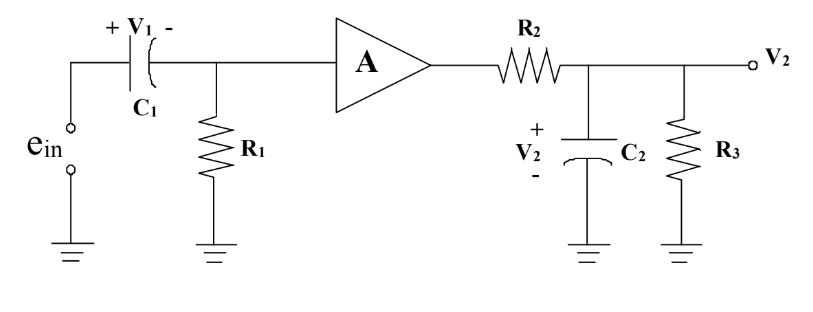
\includegraphics[scale = 0.5]{images/circuit.PNG}
    \caption{R-C Amplifier Circuit}
  \end{figure}

  Current entering through capacitor \begin{math}
    C_1
  \end{math} at the input side is:
  \begin{equation}
    C_1 \frac{dV_1}{dt} = (e_{in} - V)/R_1
  \end{equation}
  \begin{equation*}
    \frac{dV_1}{dt} = (e_{in}-V)/R_1C_1
  \end{equation*}
  Current entering through capacitor \begin{math}
    C_2
  \end{math} at the output side is:
  \begin{equation}
    C_2 \frac{dV_2}{dt} = \frac{A}{R_2(e_{in}-V1)} - \frac{V_2(R_2+R_3)}{R_2 R_3}
  \end{equation}
  Thus the equations for simulation was :
  \begin{equation}
    \frac{dV_1}{dt} = A_{11} * V_1 + B_1 * e_{in}
  \end{equation}
  \begin{equation}
    \frac{dV_2}{dt} = A_{21} * V_1 + A_{22} * V_2 + B_2 * e_{in}
  \end{equation}
  where,
  \begin{equation*}
    A_{11} = -1/(R_1C_1) = -B_1
  \end{equation*}
  \begin{equation*}
    A_{21} = -A/(R_2C_2) = -B_2
  \end{equation*}
  \begin{equation*}
    A_{22} = - (R_2 + R_3)/(R_2R_3C_2)
  \end{equation*}
  Thus the above equations become:
  \begin{equation}
    \frac{dV_1}{dt} = A_{11} * V_1 - A_{11} * e_{in} \label{eq:l2V1}
  \end{equation}
  \begin{equation}
    \frac{dV_2}{dt} = A_{21} * V_1 + A_{22} * V_2 - A_{21} * e_{in} \label{eq:l2V2}
  \end{equation}
  These values for \begin{math}
    V_1 \ and \ V_2
  \end{math}
  was solved by using Runge-Kutta-4 methods.
  \begin{equation*}
      m_1 = f(x_1,y_1)
  \end{equation*}
  \begin{equation*}
    m_2 = f(x_1 + h/2, y_1 + m_1 h/2)
  \end{equation*}
  \begin{equation*}
    m_3 = f(x_1 + h/2, y_1 + m_2 h/2)
  \end{equation*}
  \begin{equation*}
    m_4 = f(x_1 +h, y_1 + m_3 h)
  \end{equation*}
  \begin{equation*}
    y_{i+1} = y_i + ( (m_1 + 2m_2 + 2m_3 + m_4)/6)h
  \end{equation*}
  For this study,  the constants were taken as:\\
  \begin{math}
  h = 0.0002\\
  A11 = -50 sec^{-1}\\
  A21 = -10000 sec^{-1}\\
  A22 = -21.5 sec^{-1}\\
  \end{math}
  This experiment was done with n = 500 (data points).
  \cite{lab2}
  \subsection{Results}
  \subsubsection*{Case 1 : V1[0] = V2[0] = 0 and ein = 5V}
  The voltage characteristics obtained from the mathematical model of the circuit are:\\
  For V1 and V2,\\
  \begin{figure}[ht]
    \centering
    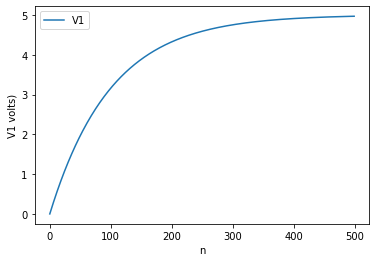
\includegraphics[scale = 0.44]{images/Exp2_Example1_V1.png}
    \caption{V1 characteristics}
  \end{figure}
  \begin{figure}[h!]
    \centering
    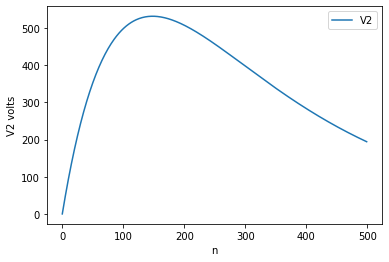
\includegraphics[scale = 0.5]{images/Exp2_Example1_V2.png}
    \caption{V2 characteristics}
  \end{figure}
  \\The mathematical model predicts that for the sampled time period, capacitor (C1) keeps on charging whereas capacitor(C2) charges at first and then discharges. 
  \subsubsection*{Case 2 : V1[0] = V2[0] = 0 and ein = -5V}
  The voltage characteristics obtained from the mathematical model of the circuit are:\\
  For V1 and V2,\\
  \begin{figure}[ht]
    \centering
    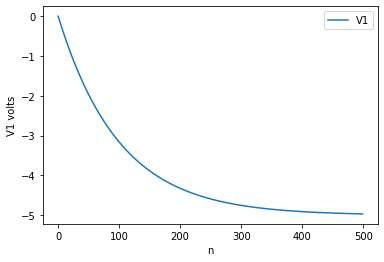
\includegraphics[scale = 0.44]{images/Exp2_Example2_V1.png}
    \caption{V1 characteristics}
  \end{figure}
  \\
  \begin{figure}[h!]
    \centering
    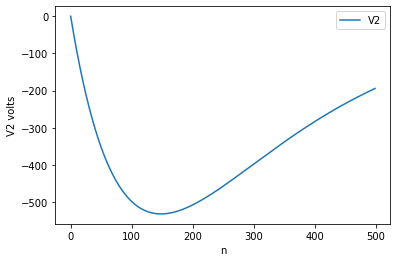
\includegraphics[scale = 0.5]{images/Exp2_Example2_V2.png}
    \caption{V2 characteristics}
  \end{figure}
  \\In this case, the polarity of input voltage is changed while keeping other parameters same. The mathematical model predicts that for the sampled time period, capacitor (C1) keeps on discharging whereas capacitor(C2) discharges at first and then charges.
  \subsection{Discussion}
  The characteristics of V1 and V2 in Case II is same as Case I but on opposite polarity.
  This is the required behaviour as only the polarity of input voltage is changed from Case I.
  Thus, this model satisfies the theoritical data that when the polarity of input voltage is reversed,
  the voltage characteristics of the circuit is also mirrored.  
  
\section{Experiment 3 : Generation of random number}
\subsection{Objective}
  \begin{itemize}
    \item To generate a Random number
  \end{itemize}
\subsection{Methodology}
  In this study, we generate a random number and use Chi-square test to veify the acceptance.
  The number is generated by Congruence method which is pseudorandom number generation. 
  In this method, we used a seed \begin{math}
    (r_o)
  \end{math} and two variables( a and b ) to generate the pseudorandom number.
  Considering P as the upper limit of random number, we got a random number in the closed interval.
  The mathematical model is given by :
  \begin{equation}
    r_{i+1} = (a * r_i + b) \%  P
  \end{equation}
  Here,
  \begin{itemize}
    \item a = 1, the method is additive.
    \item b = 0, the method is multiplicative.
    \item Else, the method is mixed. 
  \end{itemize}
  After generation of pseudorandom number, we used Chi-square test to verify the acceptance.
  Chi-square test is a frequency test given by,
  \begin{equation}
    \chi _o ^2 = \sum (O_i - E_i)^2 / E_i
  \end{equation}
  where 
  \begin{math}
    E_i = N/n
  \end{math}
  is the expected number.\\
  and \begin{math} O_i \end{math}  is the observed number.\\
  For this study, we take confidence level at \begin{math}
    \alpha = 0.005
  \end{math} and the degree of freedom as (k - 1) where k is given by Sturges' rule i.e.
  \begin{equation}
    k = 1 + 3.3 * log_{10}n
  \end{equation}
  Taking n = 256, k = 8.947 rounded up to 9. Also, degree of freedom = 9-1 = 8.\\
  For given confidence level and degree of freedom, acceptance value is found out from table. 
  Our null hypothesis assumes the numbers are random and uniformly distributed.
  If the calculated value is greater than the table value, null hypothesis is rejected and numbers are not accepted for their uniformity of distribution.
  \cite{lab3}
  \subsection{Results}
  \subsubsection*{Case I : a = 17,b = 23,P = 256}
  In this case, a!= 1 and b!= 0. This is a mixed method.
  From calculation the calculated value for chi-square test was found to be 10.27 .\\
  $\chi_{calculated}$ = 10.27\\
  From chi-square table, the critical value at $\alpha$ = 0.05 and degree of freedom = 8 is 15.51.\\
  $\chi_{table}$ = 15.51\\
  Since $\chi_{calculated} \leq \chi_{table}$, the uniformity of the random numbers is accepted.
  \begin{figure}[h!]
    \centering
    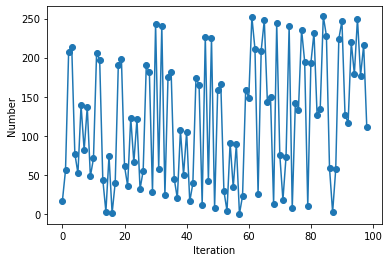
\includegraphics[scale = 0.65]{images/Exp3_Example1.png}
    \caption{Random number for a = 17, b = 23, P = 256}
  \end{figure}

  \subsubsection*{Case II : a = 1,b = 23,P = 256}
  In this case, a= 1 and b!= 0. This is a additive method.
  From calculation the calculated value for chi-square test was found to be 0.3699.\\
  $\chi_{calculated}$ = 0.3699\\
  From chi-square table, the critical value at $\alpha$ = 0.05 and degree of freedom = 8 is 15.51.\\
  $\chi_{table}$ = 15.51\\
  Since $\chi_{calculated} \leq \chi_{table}$, the uniformity of the random numbers is accepted.
  \begin{figure}[h!]
    \centering
    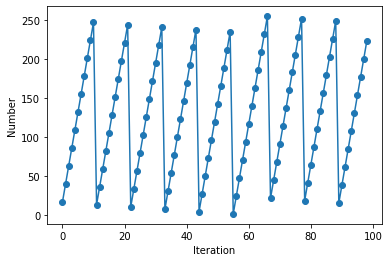
\includegraphics[scale = 0.65]{images/Exp3_Example2.png}
    \caption{Random number for a = 1, b = 23, P = 256}
  \end{figure}

  \subsubsection*{Case III : a = 17,b = 0,P = 256}
  In this case, a!= 1 and b= 0. This is a multiplicative method.
  From calculation the calculated value for chi-square test was found to be 1.0899 .\\
  $\chi_{calculated}$ = 1.0899\\
  From chi-square table, the critical value at $\alpha$ = 0.05 and degree of freedom = 8 is 15.51.\\
  $\chi_{table}$ = 15.51\\
  Since $\chi_{calculated} \leq \chi_{table}$, the uniformity of the random numbers is accepted.
  \begin{figure}[h!]
    \centering
    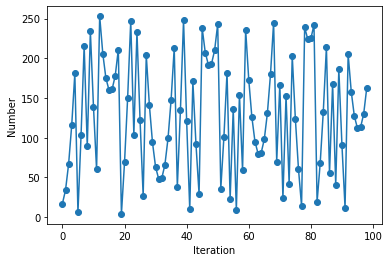
\includegraphics[scale = 0.65]{images/Exp3_Example3.png}
    \caption{Random number for a = 17, b = 0, P = 256}
  \end{figure}
\subsection{Discussion}
The random numbers generated using the congruence method were tested using the chi-square goodness of fit test at a significance level of 0.05 with degrees of freedom =8 (selected based on Sturges' rule). 
The results show that the generated numbers pass the chi-square test in all three methods i.e. additive, multiplicative and mixed. 
This indicates that they follow a uniform distribution. 
However, it's important to note that the congruence method is a pseudo-random number generator and not truly random. 
Although Case I and Case III show randomness, Case II clearly shows a repeatative pattern.
Thus, it is not appropriate for applications that require true randomness, such as cryptographic systems. 
Additionally, it's important to note that the chi-square test only tests for uniformity and does not test for other properties of randomness like independence. 
Therefore, chi-square test isn't sufficient to test if the numbers are random or not. 
Thus, further testing is needed depending on the requirement of application.

\section{Experiment 4 : Simulation of mass spring damper system}
\subsection{Objectives}
\begin{itemize}
  \item To develop the mathematical modeling of the (continuous system) mass spring damper system.
  \item To determine the state of the system i.e. x, distance moved at different point of time.
\end{itemize}  
\subsection{Methodology}
In this study, we make a mathematical model of a mass spring damper system. The physical system is as follows :
\begin{figure}[h!]
  \centering
  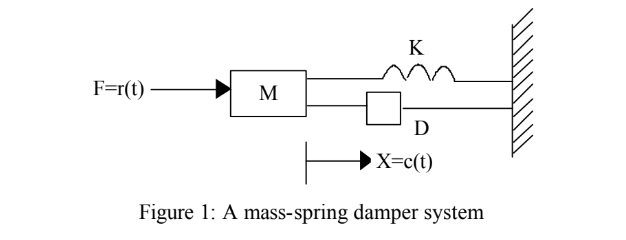
\includegraphics[scale= 0.7]{images/spring-mass.PNG}
  \caption{Mass-Spring damper system}
\end{figure}
The free body diagram of this system is :
\begin{figure}[h!]
  \centering
  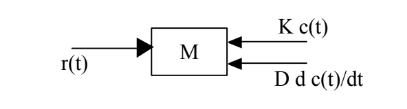
\includegraphics{images/sping_mass_freebody.PNG}
  \caption{Free-body diagram}
\end{figure}
 The mathematical model of this system can be derived from Newton's law of motion.
 \begin{equation*}
  M * \frac{d^2C(t)}{dt^2} = K r(t) - (D \frac{dC(t)}{dt} + K C(t))
 \end{equation*}
 or
 \begin{equation*}
  M * \frac{d^2C(t)}{dt^2} + D \frac{dC(t)}{dt} + K C(t) = Kr(t)
 \end{equation*}
 Thus, the mathematical model of a mass spring damper system with mass M, force r(t), damoer coefficient(D), spring coefficient(K) and displacement C(t) is given by: 
 \begin{equation}
  M * \frac{d^2C(t)}{dt^2} + D \frac{dC(t)}{dt} + K C(t) = Kr(t)
 \end{equation}
 which can be rewritten as :
 \begin{equation}
  \frac{d^2C(t)}{dt^2} + \frac{D}{M} \frac{dC(t)}{dt} + \frac{K}{M} C(t) = \frac{1}{M} Kr(t)
 \end{equation}
 This is the required mathematical model of the given mathematical system. Comparing equation 15 with general secibd order partial equation:
 \begin{equation}
  \frac{d^2x(t)}{dt^2} + 2 \xi W \frac{dx(t)}{dt} + W^2 x(t) = W^2 F
 \end{equation}
 where, Damping ratio  
 \begin{math}
  \xi = D/2 . M . W
 \end{math}
 \\Angular frequency of oscillation W = 
 \begin{math}
  \sqrt{K/M}
 \end{math} 
 \\We show how x varies in response to a steady force applied at time t = 0 for the various values of \begin{math}
  \xi .
 \end{math}
 \cite{lab4}
 \subsection{Results}
 \begin{figure}[h!]
  \centering
  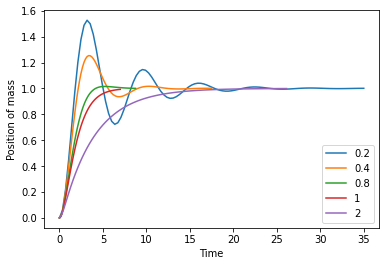
\includegraphics[scale= 0.5]{images/Exp4.png}
  \caption{Position of mass at different damping coefficients.}
 \end{figure}
 Shown above is the result of this experiment.
 The resulting graph shows the response of a spring-mass-damper system for different values of damping ratio. 
 The horizontal axis represents time, and the vertical axis represents the system's response.
 As stated in methodology, the graph shows how x(position of mass) varies for different values of $\chi$.
 The step response is the output of the system when a unit step input is applied to it. In this case, the input is a step function that changes from 0 to 1 at t=0.
 The system's response for each value of damping ratio is represented by a different colored line on the graph. 
 As the damping ratio increases, the response of the system becomes faster and oscillations are damped more quickly.
 As the damping ratio increases from 0.2 to 4, the response of the system changes from a highly oscillatory response to a slower and less oscillatory response.
 The graph can be used to choose an appropriate damping ratio for a given application, depending on the desired response of the system.
\subsection{Discussion}
The resulting graph of this study shows that the system's response changes significantly with varying damping coefficients.
For low damping coefficients, such as 0.2 and 0.4, the system is underdamped, i.e. the amplitude of oscillation gradually decreases but the system takes a long time to settle down to its steady-state. 
Similarly, for higher damping coefficients such as 4 and 8, the system is overdamped, i.e. the amplitude of oscillation reduces more rapidly but the system also takes longer to settle down.
Finally, at a damping coefficient of 1, the system shows critical damping, i.e. the system settles down to its steady-state as quickly as possible without overshooting. 
This is the optimal damping coefficient for the system since it is the most stable response.

Overall, the simulation results show that the damping coefficient plays a crucial role in the behavior of the spring-mass damper system. 
This information can be used to select appropriate damping coefficients for various systems, based on the desired response time, stability, and performance.

\section{Experiment 5 : Simulation of national econometric system}
\subsection{Objectives}
\begin{itemize}
  \item To develop the mathematical modeling of the national econometric system.
  \item To determine the state of the system at various fixed interval of time using distributed lag model
\end{itemize}
\subsection{Methodology}
  In this study, we model a national econometric system as a distributed lag model. Models that have the properties of changing only at fixed intervals of time, and of basing current values  of the variables on other current values and values that occurred in previous intervals, are called distributed lag models. Such type of models consists of linear algebra. They represent a continuous system, but one in which the data is only available at fixed
  points in time.

  For this study, following simple static mathematical model of nation econometric system is considered.
  \begin{equation}
    C = 20 + 0.7 (Y-T)
  \end{equation}
  \begin{equation}
    I = 2 + 0.1 Y
  \end{equation}
  \begin{equation}
    T = 0.2 Y
  \end{equation}
  \begin{equation}
    Y = C + I + G
  \end{equation} 
    where,\\
    C is Consumption\\
    I is Investment\\
    T is Taxes\\
    G is Government expenditure\\
    Y is national income\\
    
    This study uses above equations and simulates a basic Keynesian model of a closed economy using a simple algorithm to generate random values for government expenditure (G) and compute the values of other macroeconomic variables i.e. national income (Y), consumption (C), investment (I), and taxes (T) based on the generated values of G.
    
    This static model is made dynamic by picking a fixed time interval and expressing the
    current values of the variables in terms of values at previous interval. Any variables that appears in the form of its previous interval is said to be a lagged variable. Its values in a previous interval is denoted by attaching the suffix –1 to the variable. The static model can be made dynamic by lagging all the variables. To achieve this, we don't lag all the variables but rather we lag one variable(Y) and express all other in terms of that variable.
    Thus, above set of equations can be written as : 
    \begin{equation}
      Y = 45.45 + 2.27 (I + G)
    \end{equation}
    \begin{equation}
      I = 2 + 0.1 Y_(-1)
    \end{equation}
    \begin{equation}
      T = 0.2 Y
    \end{equation}
    \begin{equation}
      C = 20 + 0.7 ( Y - T )
    \end{equation}
    We have 5 variables (C,I,T,G,Y) and only 4 equations, thus we provide the value of G and solve the above equations. 
    \cite{lab5}
    \subsection{Result}
    \begin{figure}[h!]
      \centering
      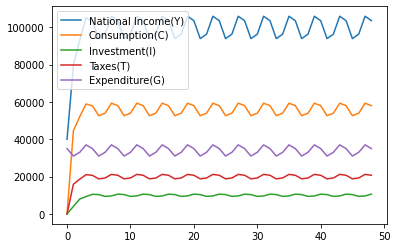
\includegraphics[scale = 0.5]{images/Exp5_Example1.png}
      \caption{Keynesian model of economy}
    \end{figure}

    \begin{figure}[h!]
      \centering
      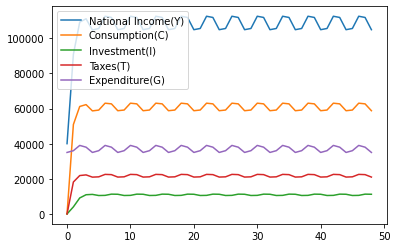
\includegraphics[scale = 0.5]{images/Exp5_Example2.png}
      \caption{Keynesian model of economy}
    \end{figure}
    The output graphs show that as the value of government expenditure (G) increases over time, there is a corresponding increase in national income (Y) and  consumption (C). 
    However, the taxes (T) and investment (I) increase only marginally, resulting in an increase in the budget deficit. 
    Similarly, the converse is also true. As G decreases, there is a decrease in Cand Y but only marginal decrease in I and T.
    Overall, the graphs show that there is a positive relationship between government expenditure and economic activity in this basic Keynesian model. 
    \subsection{Discussion}
    At Year 0, all of the variables are initialized to zero except for the lag term (G), which takes an initial value of 35,000 and national income(Y) at 40000.
    As the model evolves, the lag variable causes the other variables to fluctuate over time. 
    Some variables (C and Y) respond more strongly to G than others (I and T).

    Overall, the model presented in the code is a very simple one, and its assumptions are likely to be violated in many real-world contexts. 
    It just provides a useful starting point for thinking about the dynamics of economic variables, and highlights some of the key relationships in economic cycle.
    However, there are some limitations to the model, such as the assumption of a closed economy and the lack of consideration for inflation and other macroeconomic factors.


  \section{Conclusion}
  In conclusion, the five simulation experiments conducted in this study have demonstrated the potential of mathematical modeling and computer simulation in various fields of science and engineering. The simulation of chemical reaction has provided insights into reaction kinetics which can aid in the design of chemical reactors and optimization of chemical processes. The simulation of R-C amplifier circuit has shown the effectiveness of circuit analysis techniques and numerical methods in designing and analyzing electronic circuits. The generation of acceptable pseudo random numbers has importance in Monte Carlo simulations and stochastic modeling. The modeling of mass-spring-damper system has revealed the dynamic behavior of mechanical systems and the effects of damping and resonance on the system response. The simulation of national econometric system has demonstrated the usefulness of macroeconomic models in policy analysis and decision-making.  Overall, the study has provided valuable insights into the use of computational modeling and simulation in various applications and has highlighted the importance of numerical methods and simulation tools in modern science and engineering. 

  \section{Acknowledgement}
  The authors would like to thank Prof. Dr. Subarna Shakya,Professor, DoECE for his guidance in the classroom and for the preparation of lab sheets. 
  The authors would also like to thank Mr. Bikal Adhikari, Part-time Lecturer, DoECE for his guidance during lab hours.
  Finally, the authors are grateful to Department of Electronics and Computer Engineering guiding us through this report from start to finish.
  
  
  \renewcommand{\bibname}{References}
  \bibliographystyle{IEEEtran}
  \bibliography{ref}

  \appendices
\section{MATLAB Code for Chemical Kinetics}
\begin{verbatim}
clf
dt=0.01;
t=0:dt:1;
n=length(t);

K1=1;
K2=1;

C1=zeros(n);
C2=zeros(n);
C3=zeros(n);

C1(1) = 12;
C2(1) = 7;
C3(1) = 3;
for i=2:n
    dC = (K2*C3(i-1)-K1*C1(i-1)*C2(i-1))*dt;
    C1(i)=C1(i-1) + dC;
    C2(i)=C2(i-1) + dC;
    C3(i)=C3(i-1) - 2 * dC;
end

plot(t, C1, 'g', t, C2, 'b', t, C3, 'r');
legend('C1', 'C2', 'C3');
\end{verbatim}

\section{Python Code for Chemical Kinetics}
\begin{verbatim}
import matplotlib.pyplot as plt
import numpy as np

n = 100
dt= 1/n

C1 = [5]
C2 = [2]
C3 = [1]

K1 = 1
K2 = 1
for i in range(1,n):
    dC = (K2*C3[i-1]-K1*C1[i-1]*C2[i-1])*dt;
    C1.append(C1[i-1]+ dC)
    C2.append(C2[i-1]+ dC)
    C3.append(C3[i-1]- 2* dC)

fig = plt.figure()
plt.plot(C1, label = "C1")
plt.plot(C2, label = "C2")
plt.plot(C3, label = "C3")
    
plt.legend()
plt.show()    
\end{verbatim}

\section{MATLAB code for R-C Amplifier Circuit}
\subsubsection*{Main Code}
\begin{verbatim}
h=0.0002;
v10=0.0;
v20=0.0;
n = 500
a11=-50;
a21=-10000;
a22=-21.5;

ein = 2

v1=zeros(1,n);
v2=zeros(1,n);
t=zeros(1,n);

for i=1:n
  m11=func1(a11,v10,ein);
  m12=func1(a11,v10+m11*h/2,ein);
  m13=func1(a11,v10+m12*h/2,ein);
  m14=func1(a11,v10+m13*h,ein);
  v11=v10+((m11+2*m12+2*m13+m14)/6)*h;
  v1(i)=v11;
        
  m21=func2(v10,v20,a21,a22,ein);
  m22=func2(v10+h/2,v20+m21*h/2,a21,a22,ein);
  m23=func2(v10+h/2,v20+m22*h/2,a21,a22,ein);
  m24=func2(v10+h,v20+m23*h,a21,a22,ein);
  v21=v20+((m21+2*m22+2*m23+m24)/6)*h;
  v2(i)=v21;
        
  t(i)=h*i;
  v10=v11;
  v20=v21;
end
subplot(2,1,1)
plot(t,v1)

subplot(2,1,2)
plot(t,v2)
\end{verbatim}

\subsubsection*{func1}
\begin{verbatim}
function f1=func1(a11,v10,ein)
  f1=a11*v10-a11*ein;
end
\end{verbatim}

\subsubsection*{func2}
\begin{verbatim}
function f2=func2(v10,v20,a21,a22,ein)
  f2=a21*v10+a22*v20-a21*ein;
end
\end{verbatim}
\section{Python code for R-C Aplifier Circuit}
\begin{verbatim}
import matplotlib.pyplot as plt
import numpy as np

# Constants
h = 0.0002
a11 = -50
a21 = -10000
a22 = -21.5
n = 500

# Variables
ein = 0
V1 =[10]
V2 = [100]

def function1(v1):
  return a11*v1-a11*ein;
def function2(v1,v2):
  return a21*v1+a22*v2-a21*ein;

for i in range(0,n-1):
  m11 =function1(V1[i])
  m12 =function1(V1[i]+m11*h/2)
  m13 =function1(V1[i]+m12*h/2)
  m14 =function1(V1[i]+m13*h)
  V1.append(V1[i]+(m11+2*m12+2*m13+m14)/6*h)

  m21 =function2(V1[i],V2[i])
  m22 =function2(V1[i]+h/2,V2[i]+m21*h/2)
  m23 =function2(V1[i]+h/2,V2[i]+m22*h/2)
  m24 =function2(V1[i]+h,V2[i]+m23*h)
  V2.append(V2[i]+(m21+2*m22+2*m23+m24)/6*h)

fig = plt.figure()
plt.xlim([0,n-1])
plt.plot(V1,label = "V1")
plt.legend()
plt.show()
plt.xlim([0,n-1])
plt.plot(V2,label ="V2")
plt.legend()
plt.show()
\end{verbatim}

\section{MATLAB code for Random Number Generation}
\begin{verbatim}
clf
clearvars
a=7;
b=21;
P=64;

r(1)=17;
N = 64
for i=1:N-1
    r(i+1) = mod(r(i)*a+b,P)
end
x = 1:N
hold on
plot(x,r)
scatter(x,r)
hold off

n = 8
Ei = N/n
Oi = zeros(1,n)
h = P/n
for i=1:N
    j = floor(r(i)/h)+1
    Oi(j)= Oi(j)+1
end
x2 = 0
for i = 1:n
    x2 = x2+ ((Oi(i) - Ei)^2)/Ei
end
\end{verbatim}

\section{Python code for Random Number Generation}
\begin{verbatim}
  import matplotlib.pyplot as plt
import numpy as np
from math import log

# Variables
a = 17
b = 23
P = 256
r=[17] #seed
N = 100

for i in range (1,N-1):
    r.append((r[i-1]*a+b) % P)

x = [ i for i in range(len(r))]
fig = plt.figure()
plt.plot(r)
plt.scatter(x,r)
plt.show()

n = 9
Ei = N/n
Oi = [0] * n
h = P/n 
x2=0
for i in range(0,N-1):
    j = int(r[i]/h)
    Oi[j]= Oi[j]+1

x2 = 0
for item in Oi:
    x2 = x2 + (pow(item - Ei,2))/Ei
print(x2)
\end{verbatim}
\section{Chi-Square Table}
\begin{table}[h!]
  \centering
\begin{tabular}{| L{0.5cm} | L{1.5cm} | L{1.5cm} | L{1.5cm} | L{1.5cm} |}
  \hline
  \textbf{df/{$\alpha$}} & \textbf{0.995} & \textbf{0.99} & \textbf{0.975} & \textbf{0.95} \\ \hline
  1 & 3.84 & 6.63 & 10.83 & 16.92 \\ 
  2 & 5.99 & 9.21 & 13.82 & 21.92 \\ 
  3 & 7.81 & 11.34 & 16.27 & 24.72 \\ 
  4 & 9.49 & 13.28 & 18.47 & 27.68 \\ 
  5 & 11.07 & 15.09 & 20.52 & 30.19 \\ 
  6 & 12.59 & 16.81 & 22.46 & 32.67 \\ 
  7 & 14.07 & 18.48 & 24.32 & 35.01 \\ 
  8 & 15.51 & 20.09 & 26.12 & 37.16 \\ 
  9 & 16.92 & 21.67 & 27.88 & 39.25 \\ 
  10 & 18.31 & 23.21 & 29.59 & 41.25 \\ \hline
  \end{tabular}
\end{table}


\section{MATLAB code for simulation of mass-spring damper system}
\begin{verbatim}
clf
clearvars

k = 10;
m = 10;
D = [4 8 16 20 40 80];
for i=1:6
    A = [0 1;-k/m -D(i)/m];
    B = [0;k/m];
    C = [1 0];
    E = [0];
    my_ss = ss(A,B,C,E);
    hold on;
    step(my_ss);
end
legend ('0.2','0.4','0.8','1','2','4')
\end{verbatim}

\section{Python code for mass-spring damper system}
\begin{verbatim}
import matplotlib.pyplot as plt
from scipy import signal

#constants
k = 10
m = 10
D = [4, 8, 16, 20, 40, 80]

for i in range(0,5):
    A = [[0, 1], [-k/m, -D[i]/m]]
    B = [[0], [k/m]]
    C = [1, 0]
    E = [0]
    my_ss = signal.StateSpace(A, B, C, E)
    plt.xlabel('Time')
    plt.ylabel('Position of mass')
    t, y = signal.step(my_ss)
    plt.plot(t, y)

plt.legend(['0.2,'0.4','0.8','1','2','4'])
\end{verbatim}

\section{MATLAB Code for Simlation of national econometric system}
\begin{verbatim}
  clf
clearvars

G(1)=35000;
N = 50

for i=1:N-1
    G(i+1) = mod(G(i)*27+1000,10000)+30000
end

Y(1)=50000;
for k= 2:N
  I(k) = 2+0.1*Y(k-1);
  Y(k) = 45.45+2.27*(I(k)+G(k));
  T(k) = 0.2*Y(k);
  C(k) = 20+0.7*(Y(k)-T(k));
end
plot(Y)
hold on
plot(C)
hold on
plot(I)
hold on
plot(T)
hold on
plot(G)
h=legend('National Income(Y)','Consumption(C)',
'Investment(I)','Taxes(T)','Expenditure(G)');
\end{verbatim}

\section{Python code for National econometric system}
\begin{verbatim}
import matplotlib.pyplot as plt

G=[35000];
N = 50
for i in range (1,N-1):
    G.append(((G[i-1]*2+1000) % 10000)+30000)

Y = [40000]
I = [0]
T = [0]
C =[0]

for j in range(1,N-1):
    I.append(2+0.1*Y[j-1])
    Y.append(45.45+2.27*(I[j]+G[j]))
    T.append(0.2*Y[j])
    C.append(20+0.7*(Y[j]-T[j]))

fig = plt.figure()
plt.plot(Y,label="National Income(Y)")
plt.plot(C,label="Consumption(C)")
plt.plot(I,label="Investment(I)")
plt.plot(T,label="Taxes(T)")
plt.plot(G,label="Expenditure(G)")
plt.legend()
plt.show()
\end{verbatim}
% \bibliographystyle{IEEEtran}
% \bibliography{references}


\end{document}